\subsubsection{Local Service Review}	
The following use cases pertain to the review of service settings and logs of Condenser. Figure~\ref{LocalServiceReviewUse} shows a diagram depicting the relationships between the Local service review use cases.
\begin{center}
	\begin{figure}[htbp]
		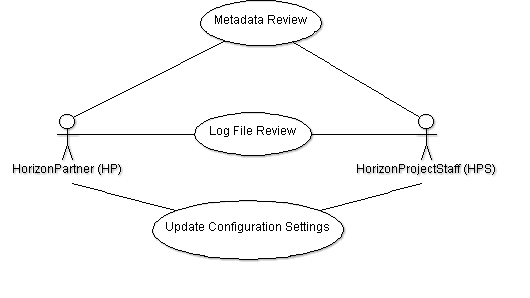
\includegraphics[scale=.5]{images/LocalServiceReviewUse.png}
		\caption{Use cases defining Condenser service review.\label{LocalServiceReviewUse}}
	\end{figure}
\end{center}	
\textbf{Use Cases:}\\
	 
	\textbf{Metadata Review} \\	 
	\textbf{Participating Actors:} Horizon Project Staff(HPS) and/or Horizon Partner (HP)\\
	\textbf{Event Flow:}
	\begin{enumerate}
\item HPS or HP accesses the metadata settings web interface for the given device. 
\item HPS or HP re-configures Condenser's provenance settings.
\item HPS or HP adds any special metadata for the given project or application.
\item Condenser's new settings are saved as a new version. Old versions are archived for future inspection.
    \end{enumerate}
	\textbf{Entry Conditions:} Condenser is running and can be connected to through the Internet.\\
	\textbf{Exit Conditions:} Condenser has new provenance settings.\\
	\textbf{Quality Requirements:} Metadata is maintained under version control.\\
	\line(1,0){350}		
			 
	\textbf{Log Review} \\	 
	\textbf{Participating Actors:} Horizon Project Staff(HPS) and/or Horizon Partner (HP) \\
	\textbf{Event Flow:}
	\begin{enumerate}
\item HPS accesses the logging settings web interface for the given device. 
\item HPS re-configures the logging settings.
\item HPS tests to make sure that activity is being logged appropriately.
    \end{enumerate}
	\textbf{Entry Conditions:} Condenser is running and can be connected to through the Internet.\\
	\textbf{Exit Conditions:} Condenser's logging settings are updated.\\
	\line(1,0){350}			
			 
	\textbf{Update configuration settings} \\	 
	\textbf{Participating Actors:} Horizon Project Staff(HPS) and/or Horizon Partner (HP) \\
	\textbf{Event Flow:}
	\begin{enumerate}
\item HPS accesses the configuration settings web interface for the given device. 
\item HPS re-configures the settings.
    \end{enumerate}
	\textbf{Entry Conditions:} Condenser is running and can be connected to through the Internet.\\
	\textbf{Exit Conditions:} Condenser's settings are updated.\\
	\line(1,0){350}			